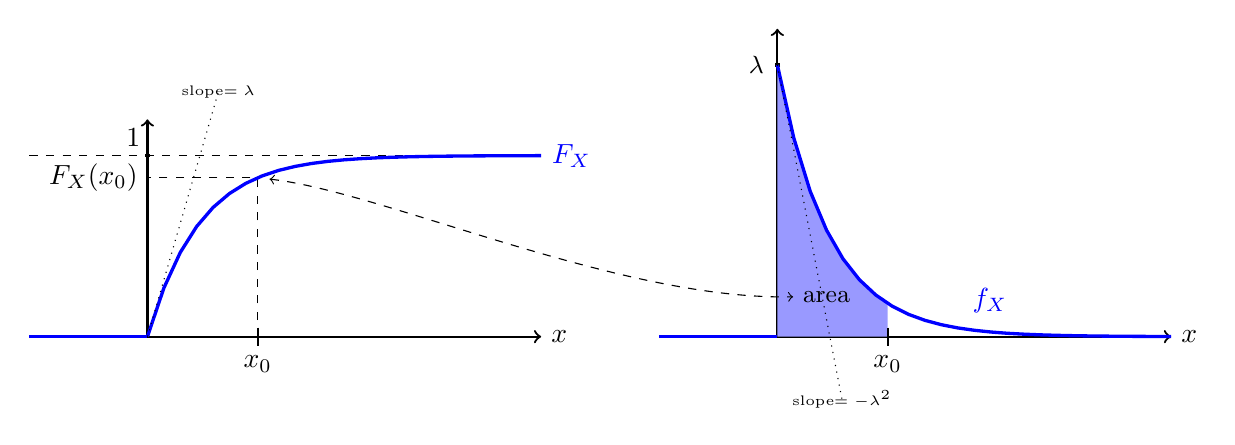
\begin{tikzpicture}[yscale=2.3]
%*** First graph ***
%Axes
\draw[<->, thick] (5,0) node[right] {$x$} --  (0,0) -- (0,1.2);
\draw[thick] (-1.5,0) -- (0,0);

%Ticks
%\foreach \x in {-1,...,4}
%\draw[xshift = \x cm, thick] (0,-1pt) -- (0,1pt) node[below] {\small $\x$};
\draw[very thick] (1pt,1) -- (-1pt,1);
	\draw (-.18,1.1) node {1};
\draw[dashed] (1.4,0)  -- (1.4,0.877) -- (0,0.877) node[left]{$F_X(x_0)$};
\draw[thick] (1.4,.05) -- (1.4,-.05) node[below] {$x_0$};

%Dashed horizontal line
\draw[dashed,thin] (-1.5,1) -- (5,1);

%Graph
\draw[very thick,blue] (-1.5,0)--(0,0);
\draw[domain=0:5, very thick, blue] plot ({\x},{1-exp(-1.5*\x)}) node[right] {$F_X$};

%Slope
\draw[dotted] (0,0) --  (0.9,1.35)node{\tiny{slope$=\lambda$}};

%*** Second graph ***
\begin{scope}[xshift=8cm]
%Axes
\draw[thick] (-1.5,0) -- (0,0);
\draw[<->, thick] (5,0) node[right] {$x$} -- (0,0) -- (0,1.7);
%\foreach \x in {-1,...,4}
%	\draw[xshift = \x cm, thick] (0,-1pt) -- (0,1pt) node[below] {\small $\x$};

%Area below curve
\fill[domain=0:1.4,blue!40,variable=\x] (0,1.5) -- plot({\x},{1.5*exp(-1.5*\x)}) -- (1.4,0) -- (0,0) -- (0,1);

%Ticks
\draw[very thick] (1pt,1.5) -- (-1pt,1.5) node[left] {\small $\lambda$};
\draw[thick] (1.4,.05) -- (1.4,-.05) node[below] {$x_0$};

%Graph
\draw[very thick,blue] (-1.5,0)--(0,0);
\draw[domain=0:5, very thick, blue] plot ({\x},{1.5*exp(-1.5*\x)});
	\draw[blue] (2.7,0.2) node {$f_X$};

%Slope
\draw[dotted] (0,1.5) --  (0.82,-0.345)node{\tiny{slope$=-\lambda^2$}};

\end{scope}

%Curved long arrow
\draw[<->, dashed, thin] (1.55,0.87) .. controls (3,0.8) and (6,0.2) .. (8.2,0.22) node[right] {\small{area}};
\end{tikzpicture}
